
%\section{Non-existence of cosmic strings in the Standard Model}
%In the Standard Model, the gauge symmetry group is known to be $\text{SU}(3)_c\otimes \text{SU}(2)_L\otimes\text{U}(1)_Y$. If we consider the only scalar field known, the Higgs field $\Phi$, we know that is a field in $\text{SU}(2)_L\otimes\text{U}(1)_Y$ that experience spontaneous symmetry breaking down to $\text{U}(1)_{\text{em}}$. Therefore, the field $\Phi$ takes values in $\left(\text{SU}(2)_L\otimes\text{U}(1)_Y\right)/\text{U}(1)_{\text{em}} \simeq \text{SU(2)}$. Since $\text{SU(2)}\simeq S^3$, we classify their topological defects, and find that $\pi_1(S^3) \simeq I$, therefore no cosmic strings are allowed in the Standard Model. However, extensions to the gauge group of the Standard Model such as SU$(5)$ and effective models can provide a much richer variety of topological defects.

\section{An extension of the Standard Model}
As we saw in Section \ref{sec:globalU}, in the Standard Model U(1)$_{B-L}$ is an exact global symmetry. However, this is strange since an exact symmetry is only natural when it is local. If we promote U(1)$_{B-L}$ to be a local symmetry, we can combine it with the symmetry U$(1)_Y$ of the Standard Model associated with the weak hypercharge $Y$. We introduce an additional U(1) Abelian gauge coupling, and we call it $h'$. We define the new charge as
\begin{equation}
	Y' = 2hY + \frac{h'}{2}(B-L),
\end{equation}
where $h$ and $h'$ are coupling constants (the convention for the coefficients $2$ and $1/2$ will be convenient later). We call the gauge field of the new U$(1)_{Y'}$ symmetry $\mathcal{A}_{\mu}$, it couples to a linear combination of the charges $Y$ and $B-L$.
 
Thus, the gauge group of the Standard Model is converted to 
\begin{equation}
	SU(3)_c\times SU(2)_L\times U(1)_{Y'}.
\end{equation}
%where $h'$ is the coupling of the new gauge boson $\mathcal{A}_{\mu}$.
With the inclusion of the new gauge coupling to $\mathcal{A}_{\mu}$, a gauge anomaly emerges, which can be seen in the triangular diagram in Figure \ref{fig:anomaly}.  In the Standard Model, we have three generations of quarks, each containing two flavors. They can have one of three color charges and be left- or right-handed. Since each quark has baryon number $B=1/3$, each generation sums up to $B = 2\times 3\times 2 \times 1/3 = 4$. 
\begin{figure}
\center
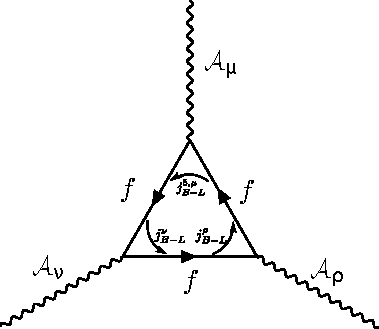
\includegraphics[scale=1]{./figures/triangularanomaly.pdf}
\caption{Triangular diagram: $f$ runs over all fermions involved. In each vertex the quarks of one generation contribute with a total baryon number $B=4$, and the leptons with total lepton number $L=3$. In order to have $\text{U}(1)_{B-L}$ gauge invariance, we introduce a right-handed neutrino with $L=1$ in each fermion generation.}
\label{fig:anomaly}
\end{figure}
In the lepton sector, each generation has one lepton with both chiralities but only a left-handed neutrino, all with $L=1$. This way, each generation contributes to the total lepton number with $L=3$.

This way, the sum of  the $B-L$ charge of one set of SM fermions does not vanish, since $B-L= 4-3=1\neq 0$.

In order to cancel the anomaly, which corresponds to the diagram  in Figure \ref{fig:anomaly}, we need the addition of a right-handed neutrino $\nu_R$ ($L = 1$). Since a right-handed neutrino is sterile, except for the $B-L$ charge, it does not affect the cancellations of other gauge anomalies with respect to the Standard Model gauge fields. It is known that we can give a Dirac mass term to the neutrinos via a Yukawa coupling through $\nu_L$ and $\nu_R$ and the standard Higgs field $\Phi$ of the form
\begin{equation}
f_{\nu} \left[\bar{\nu}_R \begin{pmatrix}-\Phi_0 & \Phi_+\end{pmatrix}\begin{pmatrix}
	\nu_L \\
	e_L
\end{pmatrix} + \begin{pmatrix}\bar{\nu}_L & \bar{e}_L\end{pmatrix}
\begin{pmatrix}
	-\Phi^*_0 \\
	\Phi^*_+
\end{pmatrix}\nu_R\right].
\end{equation}
When we set $\Phi = \begin{pmatrix}0 \\ v \end{pmatrix}$ the mass term becomes $f_{\nu}v(\bar{\nu}_R\nu_L+\bar{\nu}_L\nu_R)$ and we can read directly the mass for the neutrino $m_{\nu} = f_{\nu}v$.

The Majorana term permitted normally to give mass to the right-handed neutrino is of the form
\begin{equation}
	M\bar{\nu}_M \nu_M,
\end{equation}
where $\nu_M = \nu_R + C\bar{\nu}^T_R$, with $C$ the charge conjugation matrix. However, this term is only possible if the right-handed neutrino is completely sterile. We now have a $B-L$ gauge field, and if we want to construct a mass term solely for $\nu_R$, we add a non-standard Higgs field.
 The weak and $B-L$ charges of the Higgs fields are summarize in Table \ref{tab:charges}.
\begin{table}
\begin{center}
\begin{tabular}{|c|c|c|}
\hline 
 Charge & $\chi$ & $\Phi$ \\ 
\hline \hline
$Y$ & 0 & $\frac{1}{2}$ \\ 
\hline 
${B-L}$  & 2 & 0 \\ 
%\hline 
%$Y'={2hY+\frac{h'}{2}(B-L)}$  & $h'$ & $h$ \\ 
\hline 
\end{tabular} 
\end{center}
\caption{The hypercharges of the Higgs fields $\chi$ and $\Phi$.}% and $1/2$, respectively. On the other hand the $B-L$ charge of $\Phi$ is $0$. However, we define the $B-L$ charge of the $\chi$ to be 2 in order to retain gauge invariance.}
\label{tab:charges}
\end{table}

Moreover, we can also give a Majorana-type mass term to $\nu_R$, in\-de\-pend\-ent\-ly of $\nu_L$ through the Higgs mechanism 
\begin{equation}
\label{eq:majorana}
f_{\nu_R} \nu_R^T \chi \nu_R + \text{c.c.},
\end{equation}
where $f_{\nu_R}$ is a Yukawa coupling and in order to retain gauge invariance we added the non-standard Higgs-type field $\chi\in\mathbb{C}$.
The $B-L$ charge of this term must be zero. The neutrino fields together have $B-L = -2$, so the field $\chi$ must have a charge $B-L=2$.

\section{Lagrangian and equations of motion for U(1)$_{Y'}$ cosmic strings} 

The new Higgs field $\chi$ is introduced in the Lagrangian with a gauge invariant potential 
\begin{equation}
V' = \frac{m'^{2}}{2}\chi^*\chi+\frac{\lambda'}{4}(\chi^*\chi)^2.
\end{equation}
Because of power-counting renormalizability we only include four powers in the field $\chi$.
It can be applied to each lepton generation to give mass to all right-handed neutrinos via the Higgs mechanism according to eq.\ \eqref{eq:majorana}. We denote the vacuum expectation value of $\chi$ as $v'$.

It is also natural to include a mixed term $\propto \kappa\Phi^{\dagger}\Phi\chi^*\chi$, between the standard Higgs field and the new Higgs field. This term is natural because it is gauge invariant under both U(1)$_Y'$ and SU$(2)_L$. Again, by power counting renormalizability we only include four powers in energy, giving the coupling constant $\kappa$ dimension zero.

Furthermore, we assume the vacuum expectation value of the new Higgs field $v'$ to be much greater than the vacuum expectation value of the standard Higgs field $v$, that is, $v'\gg v$. In addition, we assume  $f_{\nu_R}\simeq O(1)$ which together gives a heavy mass to the right-handed neutrino, $m_{\nu_R} = f_{\nu_R}v'$. For simplicity, we exclude the SU$(2)_L$ gauge field and the fermion fields, along with the gluons. Therefore, the Lagrangian with these approximations reads
\begin{eqnarray} 
	\mathcal{L} & = & \frac{1}{2}(D^{\mu}\Phi)^{\dagger}D_{\mu}\Phi - \frac{m^2}{2}\Phi^{\dagger}\Phi - \frac{\lambda}{4}(\Phi^{\dagger}\Phi)^2 -\frac{\lambda}{4}v^4   \nonumber\\
 & & +\frac{1}{2}(D^{\mu} \chi)^*D_{\mu} \chi - \frac{m'^2}{2}\chi^*\chi - \frac{\lambda'}{4}(\chi^* \chi)^2 -\frac{\lambda'}{4}v'^4\nonumber \\ 
 & & -\frac{\kappa}{2}\Phi^\dagger\Phi\chi^*\chi  -\frac{\kappa}{2}v^2v'^2 -\frac{1}{4}\mathcal{F}^{\mu\nu}\mathcal{F}_{\mu\nu}, %+ \frac{1}{4}B_{\mu\nu}B_{\mu\nu}
\end{eqnarray}
where 
\begin{eqnarray}
D_{\mu} \Phi & \equiv & (\partial_{\mu} + ih\mathcal{A}_{\mu})\Phi,\nonumber \\ 
D_{\mu} \chi & \equiv & (\partial_{\mu} + ih'\mathcal{A}_{\mu})\chi,\nonumber \\
\mathcal{F}_{\mu\nu} & \equiv & \partial_{\mu}\mathcal{A}_{\nu}-\partial_{\nu}\mathcal{A}_{\mu},
\label{eq:covder}%,\\
%B_{\mu\nu} & = & \partial_{\mu}B_{\nu}-\partial_{\nu}B_{\mu}.
\end{eqnarray}
and the gauge field $\mathcal{A}_{\mu}$ is introduced to implement local U$(1)_{Y'}$ invariance. The fields transform as
\begin{eqnarray}
	\Phi(x) \to e^{ih\alpha(x)}\Phi(x), \nonumber \\
	\chi(x) \to e^{ih'\alpha(x)}\chi(x), \nonumber\\
	\mathcal{A}_{\mu} \to \mathcal{A}_{\mu} + \partial_{\mu} \alpha(x),
\end{eqnarray}
where $\alpha$ is any differentiable function of $x$.
Expanding the covariant derivative terms of eq.\ \eqref{eq:covder} we obtain
\begin{eqnarray*}
	(D^{\mu}\Phi)^{\dagger}D_{\mu}\Phi & = &  \partial^{\mu}\Phi^{\dagger}\partial_{\mu}\Phi + ih\partial^{\mu}\Phi^{\dagger}\mathcal{A}_{\mu} \Phi - ih\mathcal{A}^{\mu} \Phi^{\dagger}\partial_{\mu}\Phi +h^2\mathcal{A}^{\mu}\mathcal{A}_{\mu} \Phi^{\dagger}\Phi,\\
	 (D^{\mu}\chi)^{*}D_{\mu}\chi & = &  \partial^{\mu}\chi^{*}\partial_{\mu}\chi + ih'\partial^{\mu}\chi^{*}\mathcal{A}_{\mu} \chi - ih'\mathcal{A}^{\mu} \chi^{*}\partial_{\mu}\chi +h'^2\mathcal{A}^{\mu}\mathcal{A}_{\mu} \chi^{*}\chi.
\end{eqnarray*}
We want to derive the Euler-Lagrange equations regarding the derivatives with respect to $\Phi^{\dagger}$
\begin{eqnarray}
	\partial^{\mu}\frac{\partial \mathcal{L}}{\partial (\partial^{\mu}\Phi^{\dagger})} & = & \frac{\partial \mathcal{L}}{\partial \Phi^{\dagger}},\nonumber \\
	\frac{\partial  \mathcal{L}}{\partial (\partial^{\mu} \Phi^{\dagger})}  & = & \frac{1}{2}\partial_{\mu} \Phi + \frac{ih}{2}\mathcal{A}_{\mu}\Phi = \frac{1}{2}D_{\mu}\Phi,\nonumber \\
	\label{eq:eula_lhs}
	 \partial^{\mu}\frac{\partial \mathcal{L}}{\partial (\partial^{\mu}\Phi^{\dagger})} & = & \frac{1}{2}\partial^{\mu} \left(\partial_{\mu} + i h\mathcal{A}_{\mu}\right)\Phi = \frac{1}{2}\partial^{\mu}D_{\mu}\Phi,
\end{eqnarray}
\begin{eqnarray}
\label{eq:eula_rhs}
	\frac{\partial \mathcal{L}}{\partial \Phi^{\dagger}}  & = &  \frac{1}{2} \left[-ih\mathcal{A}^{\mu}\partial_{\mu}\Phi + h^2\mathcal{A}^{\mu}\mathcal{A}_{\mu}\Phi \right]- \frac{m^2}{2}\Phi -  \frac{\lambda}{2} (\Phi^{\dagger}\Phi)\Phi - \frac{\kappa}{2}\Phi \chi^*\chi\nonumber\\
	& = &-\frac{1}{2}ih\mathcal{A}^{\mu}D_{\mu} \Phi - \frac{m^2}{2}\Phi - \frac{\lambda}{2}  (\Phi^{\dagger}\Phi)\Phi - \frac{\kappa}{2}\Phi \chi^*\chi \ .
\end{eqnarray}
Equating \eqref{eq:eula_lhs} and \eqref{eq:eula_rhs} we obtain the equation of motion for $\Phi$
\begin{equation}
	\label{eq:phi}
	D^{\mu}D_{\mu} \Phi = -m^2 \Phi - \lambda (\Phi^{\dagger}\Phi)\Phi - \kappa \Phi \chi^* \chi \ .
\end{equation}
Similarly, we obtain the equation of motion for the field $\chi$
\begin{equation}
	\label{eq:chi}
	D^{\mu}D_{\mu} \chi = -m'^2 \chi - \lambda' (\chi^{*}\chi)\chi - \kappa \chi \Phi^{\dagger} \Phi \ . 
\end{equation}
Regarding the equations of motion of the gauge field $\mathcal{A}_{\mu}$, we first take the derivate of the Lagrangian with respect to $\mathcal{A}_{\rho}$
\begin{eqnarray}
	\frac{\partial \mathcal{L}}{\partial \mathcal{A}_{\rho}} & = & \frac{ih}{2}\partial^{\rho}\Phi^{\dagger}\Phi -\frac{ih}{2}\Phi^{\dagger}\partial^{\rho}
	 \Phi+h^2\mathcal{A}^{\rho}\Phi^{\dagger}\Phi\nonumber\\
	 & & + \frac{ih'}{2}\partial^{\rho}\chi^{*}\chi -\frac{ih'}{2}\chi^{*}\partial^{\rho}\chi+h'^2\mathcal{A}^{\rho}\chi^{*}\chi \nonumber\\
	& = & \frac{ih}{2}\left[ (D^{\rho}\Phi)^{\dagger}\Phi-\Phi^{\dagger}D^{\rho}\Phi\right] + \frac{ih'}{2}\left[ (D^{\rho}\chi)^{*}\chi-\chi^{*}D^{\rho}\chi\right].
\end{eqnarray}
Then, we take the derivative of the Lagrangian with respect to $\partial_{\lambda}\mathcal{A}_{\rho}$ 
\begin{eqnarray}
	\label{eq:maxwell}
	\frac{\partial \mathcal{L}}{\partial (\partial_{\lambda}\mathcal{A}_{\rho})} & = & \frac{\partial}{\partial (\partial_{\lambda}\mathcal{A}_{\rho})}\left(-\frac{1}{4}\mathcal{F}^{\mu\nu}\mathcal{F}_{\mu\nu}\right) \nonumber\\
	& = & -\frac{1}{4}\frac{\partial}{\partial (\partial_{\lambda}\mathcal{A}_{\rho})}\left(\partial^{\mu}\mathcal{A}^{\nu}-\partial^{\nu}\mathcal{A}^{\mu}\right)\left(\partial_{\mu}\mathcal{A}_{\nu}-\partial_{\nu}\mathcal{A}_{\mu}\right) \nonumber\\
	& = & -\frac{1}{4}\frac{\partial}{\partial (\partial_{\lambda}\mathcal{A}_{\rho})}(2\partial^{\mu}\mathcal{A}^{\nu}\partial_{\mu}\mathcal{A}_{\nu}-2\partial^{\mu}\mathcal{A}^{\nu}\partial_{\nu}\mathcal{A}_{\mu}) \nonumber\\
	& = & -\frac{1}{4}\left(2\partial^{\mu}\mathcal{A}^{\nu}\delta_{\lambda\mu}\delta_{\rho\nu}-2\partial^{\mu}\mathcal{A}^{\nu}\delta_{\lambda\nu}\delta_{\rho\mu}-2\partial^{\nu}\mathcal{A}^{\mu} \delta_{\lambda\mu}\delta_{\rho\nu}+2\partial^{\nu}\mathcal{A}^{\mu}\delta_{\lambda\nu}\delta_{\rho\mu}\right) \nonumber\\
	& = & -\frac{1}{4}(4\partial^{\lambda}\mathcal{A}^{\rho}-4\partial^{\rho}\mathcal{A}^{\lambda}) = -\partial^{\lambda}\mathcal{A}^{\rho}+\partial^{\rho}\mathcal{A}^{\lambda} = -\mathcal{F}^{\lambda\rho} = \mathcal{F}^{\rho\lambda}.
\end{eqnarray}
Differentiating the result of eq.\ \eqref{eq:maxwell} by $x_{\lambda}$ yields
\begin{equation}
\partial_{\lambda}\left(\frac{\partial \mathcal{L}}{\partial (\partial_{\lambda}\mathcal{A}_{\rho})}\right) = \partial_{\lambda}\mathcal{F}^{\rho\lambda} = \partial_{\lambda}\partial^{\rho}\mathcal{A}^{\lambda}-\partial_{\lambda}\partial^{\lambda}\mathcal{A}^{\rho}.
\end{equation}
Thus, we obtain the equations of motion  for the gauge field $\mathcal{A}_{\mu}$
\begin{equation}
\label{eq:max_eqs}
\partial_{\lambda}\mathcal{F}^{\rho\lambda} = \frac{ih}{2}\left[ (D^{\rho}\Phi)^{\dagger}\Phi-\Phi^{\dagger}(D^{\rho}\Phi)\right] + \frac{ih'}{2}\left[ (D^{\rho}\chi)^{*}\chi-\chi^{*}(D^{\rho}\chi)\right].
\end{equation}
Using cylindrical coordinates $(r,\varphi,z)$, we make ans\"{a}tze for the stationary solutions 
\begin{equation}
\Phi = \begin{pmatrix} 0 \\
  \phi(r)e^{in\varphi}\end{pmatrix},
   \ \ \ \chi = \xi(r) e^{in'\varphi}, \ \ \ \mathcal{A}^{\varphi}= \frac{a(r)}{r}.
\end{equation}
 Then, the $\varphi$ components of the covariant derivatives are
\begin{eqnarray}
	\frac{1}{r}D_{\varphi}\Phi = \left(\frac{1}{r}\partial_{\varphi} + ih\mathcal{A}_{\varphi}\right)\Phi, \nonumber \\
	 \frac{1}{r}D_{\varphi}\chi = \left(\frac{1}{r}\partial_{\varphi} + ih'\mathcal{A}_{\varphi}\right)\chi ,
\end{eqnarray}
along with
\begin{eqnarray}
	D^iD_i \Phi\equiv \left(\partial_r^2 + \frac{1}{r}\partial_r +\left(\frac{1}{r}\partial_{\varphi}+ih\mathcal{A}_{\varphi}\right)^2 +\partial^2_z\right)\Phi, \nonumber \\
	D^iD_i \chi\equiv \left(\partial_r^2 + \frac{1}{r}\partial_r +\left(\frac{1}{r}\partial_{\varphi}+ih'\mathcal{A}_{\varphi}\right)^2 +\partial^2_z\right)\chi \ .
\end{eqnarray}
%\begin{eqnarray}
%	\left(\frac{1}{r}\partial_{\varphi}+ih\frac{a(r)}{r}\right)^2\phi e^{in\varphi} %& = & \left(\frac{1}{r}\partial_{\varphi}+ih\frac{a(r)}{r}\right)\left(\frac{1}{r}\partial_{\varphi}+ih\frac{a(r)}{r}\right)\phi e^{in\varphi} \\
%	& = & \left(\frac{1}{r}\partial_{\varphi}+ih\frac{a(r)}{r}\right)\left(\frac{1}{r}(in)\phi e^{in\varphi} +ih \frac{a(r)}{r}\phi e^{in\varphi} \right) \\
%	& = & \left(\frac{1}{r^2}(in)^2\phi e^{in\varphi}+2(in)ih \frac{a(r)}{r^2}\phi e^{in\varphi}-h^2\frac{a(r)^2}{r^2}\phi e^{in\varphi}\right) \\
%	& = & -\left(\frac{n^2}{r^2}+2nh\frac{a(r)}{r^2}+h^2\frac{a(r)^2}{r^2}\right)\phi e^{in\varphi} \\
%	\left(\frac{1}{r}\partial_{\varphi}+ih'\frac{a(r)}{r}\right)^2\xi e^{in'\varphi} & = & -\left(\frac{n'^2}{r^2}+2n'h'\frac{a(r)}{r^2}+h'^2\frac{a(r)^2}{r^2}\right)\xi e^{in'\varphi} 
%\end{eqnarray}
We now work out the left-hand side of eq.\ \eqref{eq:max_eqs}, for static configurations
\begin{eqnarray}
\label{eq:vec_rel_max}
	\partial_{\nu}\mathcal{F}^{\mu\nu}  & = & \partial_{\nu} \partial^{\mu}\mathcal{A}^{\nu}-\partial_{\nu}\partial^{\nu}\mathcal{A}^{\mu} =-\partial_j\partial^i\mathcal{A}^j+\partial^j\partial_j\mathcal{A}^i \nonumber \\
	 & = &  -\left[\nabla(\nabla\cdot \mathcal{A})\right]^i+\left[ \nabla^2 \mathcal{A}\right]^i\nonumber \\
	 & = & - \left[\nabla\times\nabla\times\mathcal{A}\right]^i.
	%&    \frac{\partial_r^2 a}{r}-\frac{\partial_r a}{r^2} \ .
\end{eqnarray}
In cylindrical coordinates, the curl of a vector function takes the form of the determinant \cite{Arfken}
\begin{equation}
	\nabla\times\vec{b} = \frac{1}{r}\begin{vmatrix}
	\hat{r} & r{\hat{\varphi}} & \hat{z} \\
	\partial_r & \partial_{\varphi} & \partial_z \\
	b^r & rb^{\varphi} & b^z 
	\end{vmatrix}.
\end{equation}
Then
\begin{eqnarray}
	\nabla\times\vec{\mathcal{A}} = \nabla\times\left( \frac{a(r)}{r}\hat{\varphi}\right) & = & \frac{1}{r} \begin{vmatrix}
	\hat{r} & r\hat{\varphi} & \hat{z} \\
	\partial_r & \partial_{\varphi} & \partial_z \\
	0 & a & 0
	\end{vmatrix} = \frac{1}{r}\partial_r a \ \hat{z}, \nonumber \quad\\
	\nabla \times \nabla \times \vec{\mathcal{A}} = \nabla \times \left(\frac{1}{r}\partial_r a \ \hat{z}\right) & = & \frac{1}{r}\begin{vmatrix}
	\hat{r} & r\hat{\varphi} & \hat{z} \\
	\partial_r & \partial_{\varphi} & \partial_z \\
	\label{eq:rel1}
	0 & 0 & \frac{1}{r}\partial_r a 
	\end{vmatrix}\nonumber \\
	& = & \left(-\frac{1}{r}\partial_r^2 a + \frac{1}{r^2}\partial_r a\right)\hat{\varphi} \quad
\end{eqnarray}
Eq. \eqref{eq:vec_rel_max} is non-trivial only for the index $j = \varphi$, where we obtain from eq.\ \eqref{eq:rel1}
\begin{equation}
	\label{eq:max_eqs_phi}
	\partial_j\mathcal{F}^{\varphi j} = \frac{1}{r}\partial_r^2 a - \frac{1}{r^2}\partial_r a.
\end{equation}
Now we treat the terms on the right-hand side of eq.\ \eqref{eq:max_eqs},
\begin{eqnarray}
%\label{eq:first_rel}
\frac{ih}{2}\left(\frac{1}{r}\partial_{\varphi}\Phi\right)^{\dagger}\Phi = \frac{ih}{2}\frac{1}{r}\partial_{\varphi}(\phi e^{-in\varphi})\phi e^{in\varphi} = \frac{hn}{2r}\phi^2 \nonumber \\ 
-\frac{ih}{2}\Phi^{\dagger}\left(\frac{1}{r}\partial_{\varphi}\Phi\right) = -\frac{ih}{2}\frac{1}{r}\partial_{\varphi}(\phi e^{in\varphi})\phi e^{-in\varphi} = \frac{hn}{2r}\phi^2 \nonumber \\
h^2 \mathcal{A}_{\varphi} \Phi^{\dagger}\Phi = h^2\frac{a}{r}\phi e^{-in\varphi}\phi e^{in\varphi} = h^2 \frac{a}{r}\phi^2 \nonumber \\
\frac{ih'}{2}\left(\frac{1}{r}\partial_{\varphi}\chi\right)^{*}\chi = \frac{ih'}{2}\frac{1}{r}\partial_{\varphi}(\xi e^{-in'\varphi})\xi e^{in'\varphi} = \frac{h'}{2} n'\frac{1}{r}\xi^2  \nonumber \\ 
-\frac{ih'}{2}\chi^{*}\left(\frac{1}{r}\partial_{\varphi}\chi\right) = -\frac{ih'}{2}\frac{1}{r}\partial_{\varphi}(\xi e^{in'\varphi})\xi e^{-in'\varphi} =\frac{h'}{2} n'\frac{1}{r}\xi^2\nonumber  \\
\label{eq:last_rel}
h'^2 \mathcal{A}_{\varphi} \chi^{*}\chi = h'^2\frac{a}{r}\xi e^{-in'\varphi}\xi e^{in'\varphi} = h'^2\frac{a}{r}\xi^2 \ .
\end{eqnarray}


From eq.\ \eqref{eq:phi} we infer the equation of motion for $\phi(r)$
\begin{equation}
	\label{eq:final_phi}
	\partial_r^2 \phi + \frac{1}{r} \partial_r \phi- \frac{1}{r^2}\left(n+ha\right)^2\phi- m^2 \phi- \lambda \phi^3-\kappa \phi \xi^2 = 0,
\end{equation}
and from eq.\ \eqref{eq:chi} we obtain
\begin{equation}
	\label{eq:final_xi}
	\partial_r^2 \xi + \frac{1}{r} \partial_r \xi - \frac{1}{r^2}\left(n'+h'a \right)^2\xi -m'^2\xi - \lambda' \xi^3 - \kappa \xi \phi^2 = 0\ .
\end{equation}
And finally from eqs.\ \eqref{eq:max_eqs_phi} and \eqref{eq:last_rel} we infer
\begin{equation}
	\label{eq:a}
\partial_r^2a -\frac{1}{r}\partial_r a-h(n+ha)\phi^2-h' (n'+h'a)\xi^2 = 0.
\end{equation}
\subsection{Boundary conditions}
In the limit $r\to \infty$, the radial profile functions $\phi$ and $\xi$ take constant values $v$ and $v'$, respectively. In the same limit, eqs.\ \eqref{eq:final_phi} and \eqref{eq:final_xi} fix the values for $m^2$ and $m'^2$. If we treat $\lambda$, $\lambda'$ and $\kappa$ as free parameters, we fix the values for $m^2$ and $m'^2$
\begin{eqnarray}
	\label{eq:meqs}
	-m^2v-\lambda v^3 - \kappa v v'^2 = 0 & \Rightarrow & m^2 = -\kappa v'^2 - \lambda v^2, \nonumber\\
	-m'^2v'-\lambda' v'^3 - \kappa v' v^2 = 0 & \Rightarrow  & m'^2 = -\kappa v^2 - \lambda' v'^2.
\end{eqnarray}
Also the value $a(r\to\infty)$ is fixed using eq.\ \eqref{eq:a}. We are interested in solutions that apply to any values of $\phi$ and $\xi$ which is only possible when the parentheses in eq.\ \eqref{eq:a} are zero in the limit $r\to\infty$. We obtain the limit
\begin{equation}
\lim_{r\to \infty}a(r) \equiv a(\infty) = -\frac{n}{h}=-\frac{n'}{h'}.
\label{eq:goodlimit}
\end{equation} 
In addition, there exists another limit of $a$ at infinity
%\begin{equation}
%\partial_r^2a -\frac{1}{r}\partial_r a-h(n+ha)\phi^2-h' (n'+h'a)\xi^2 = 0
%\end{equation}
%so at $r\to \infty$, the value of $a$ is fixed only if we have
\begin{equation}
	-hnv^2 - h^2a(\infty)v^2 - h' n' v'^2 - h'^2 a(\infty) v'^2 = 0 \ \ \Rightarrow  \ \ a(\infty) = -\frac{hnv^2+h'n' v'^2}{h^2v^2+h'^2 v'^2}.
	\label{eq:badlimit}
\end{equation}
We reject the limit in eq.\ \eqref{eq:badlimit} because we demand the function $a$ to be independent of $v$ and $v'$. In contrast, the limit of \eqref{eq:goodlimit} is valid for any $\phi$ and $\xi$ which are constant at $r\to\infty$.


In summary, the boundary conditions for $\phi$, $\xi$, $a$ and  for $n,\ n' > 0$ are 
\begin{eqnarray}
	\phi(0)=0, & \displaystyle\lim_{r\to\infty}\phi(r) = v \nonumber \\
	 \xi(0)=0, &  \displaystyle\lim_{r\to\infty}\xi(r) = v' \nonumber  \\
	 a(0)=0, & \displaystyle \lim_{r\to\infty}a(r) = -\frac{n}{h}=-\frac{n'}{h'}\ .
\end{eqnarray}
For $n=0$ or $n'=0$, $\phi(0)\neq 0$ or $\xi(0) \neq 0$ is possible, respectively.

\subsection{Condition on $\kappa$}

We know that for the potential to be bounded from below, the constants $\lambda$ and $\lambda'$ must be both positive.

We now study the conditions on the Higgs-Higgs coupling $\kappa$. The potential term involving the Higgs fields is
\begin{equation}
V(\Phi,\chi) = \frac{m^2}{2}\Phi^{\dagger}\Phi+\frac{m'^2}{2}\chi^{*}\chi+\frac{\lambda}{4}(\Phi^{\dagger}\Phi)^2+\frac{\lambda'}{4}(\chi^{*}\chi)^2+\frac{\kappa}{2}\Phi^{\dagger}\Phi\chi\chi^*,
\end{equation}
where $m^2<0$ and $m'^2<0$.

To take a general perspective, it is convenient to study the concavity of the function
\begin{equation}
V(x,y) = ax^2 + by^2+cx^4+dy^4+ex^2y^2
\end{equation}
where $a,b<0$ and $c,d>0$. However, if we demand $V$ to be bounded from below it is not sufficient that $c,d>0$; we need a condition for $e$. The Hessian matrix of $V(x,y)$ reads
$$H=\begin{pmatrix}
2a+12cx^2+2ey^2 & 4exy \\
4exy & 2b+12dy^2+2ex^2 
\end{pmatrix},$$
and the gradient is
$$\nabla V = \begin{pmatrix}
2ax+4cx^3+2exy^2 \\
2by+4dy^3+2ex^2y
\end{pmatrix}.$$
From the gradient we note that the point $(0,0)$ is a critical point of $V$. At this point the Hessian takes the form
$$H(0,0)=\begin{pmatrix}
2a & 0 \\
0 & 2b
\end{pmatrix}.$$
Since the eigenvalues of $H$ at $(0,0)$ are both negative, we know that the function $V$ is concave, hence $(0,0)$ is a local maximum.
There are other critical points: those points must be local minima or saddle points for $V$ since we demand $V$ to be bounded from below and we already found the only local maximum. In order to study them, we perform the coordinate transformation
\begin{equation}
	X = x^2, \ \ \ \ Y =y^2.
	\label{eq:changeofcoor}
\end{equation}
The potential becomes
\begin{equation}
V(X,Y) = aX + bY+cX^2+dY^2+eXY.
\end{equation}
The gradient is zero when 
\begin{eqnarray}
2cX + eY & = & -a \\
eX + 2dY & = & -b
\end{eqnarray}
with the solution
\begin{eqnarray}
X_c & = & \frac{-2ad+be}{4cd-e^2}, \\
Y_c & = & \frac{-2bc+ae}{4cd-e^2}.
\end{eqnarray}
The Hessian matrix of $V$ for this coordinate transformation, evaluated at this critical point, is
\begin{equation}
H=\begin{pmatrix}
2c & e \\
e & 2d
\end{pmatrix}.
\end{equation}
Focusing on the local minima of the function, we know that in this case $\det H>0$ and $\frac{\partial^2 V}{\partial X^2} = 2c > 0$, see \cite{Marsden2012}. Due to eq.\ \eqref{eq:changeofcoor} both $X_c$ and $Y_c$ are positive quantities, and since the determinant is positive for the minima, that means that the numerators are also positive, which implies
\begin{equation}
	e<\frac{2ad}{b} ,\ \ \ e<\frac{2bc}{a},
\end{equation}
and
\begin{equation}
	\det H = 4cd - e^2 > 0 \ \ \ \Rightarrow  \ \ \ e^2 < 4cd.
\end{equation}
If we substitute
$$a = \frac{m^2}{2}, \ \ \  b = \frac{m'^2}{2}, \ \ \  c = \frac{\lambda}{4}, \ \ \  d = \frac{\lambda'}{4}, \ \ \ e = \frac{\kappa}{2},$$
then we have conditions on $\kappa$
\begin{equation}
-\sqrt{\lambda \lambda'} < \kappa < \sqrt{\lambda \lambda'},
\end{equation}
and
\begin{equation}
	{\kappa} < \frac{m^2\lambda'}{m'^2}, \ \ \ {\kappa} < \frac{m'^2\lambda}{m^2}.
	\label{eq:redundant}
\end{equation}
We combine all the conditions as follows
\begin{equation}
	-\sqrt{\lambda \lambda'} < \kappa < \min \left(\sqrt{\lambda \lambda'},\frac{m'^2\lambda}{m^2},\frac{m^2\lambda'}{m'^2}\right).
\end{equation}
However, the inequalities in eq.\ \eqref{eq:redundant} are redundant. We take the values for $m^2$ and $m'^2$ from eq.\ \eqref{eq:meqs} and substitute them in one of the inequalities. Working with the first one in  eq.\ \eqref{eq:redundant} and recalling that $m^2,\ m'^2 <0$, we obtain
\begin{eqnarray}
	{\kappa} & < & \frac{-\kappa v'^2 - \lambda v^2}{-\kappa v^2 - \lambda' v'^2}\lambda'\nonumber \\
	& = & \frac{\kappa v'^2 + \lambda v^2}{\kappa v^2 + \lambda' v'^2}\lambda' \nonumber \\
	\kappa^2v^2+\kappa\lambda' v'^2 & < & \kappa\lambda' v'^2 + \lambda\lambda' v^2 \nonumber\\
	\kappa^2 & < & \lambda\lambda'. 
\end{eqnarray}
Similarly, we obtain the same result when we work out the second inequality in eq.\ \eqref{eq:redundant}. We are left with only one condition
\begin{equation}
 \boxed{\kappa^2 < \lambda \lambda'}\ .
\end{equation}


%Figures \ref{fig:1}, \ref{fig:2}, \ref{fig:3} and \ref{fig:4} show the solutions for the functions $\phi$, $\xi$ and $a$ for various values of $n$, $n'$, $h$, $h'$, $\lambda$, $\lambda'$ in the range $\kappa\in[-2,2]$ and $\kappa\in[-1.5,1.5]$ for figure \ref{fig:3}. 
%
%
%\begin{figure}
%\centering
%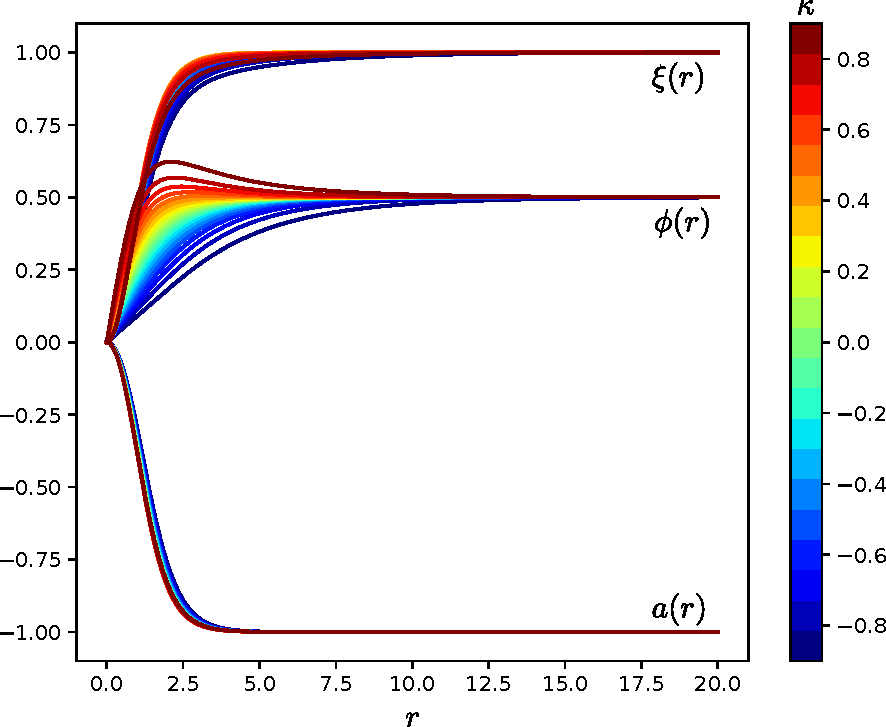
\includegraphics[scale=1]{./figures/Figure_1.pdf}
%\caption{$h=n=0$, $h'=n' = 1$, $\lambda=\lambda'=1$, $v=0.1$, $v'=1/4$ and $\kappa\in [-2,2]$.}
%\label{fig:1}
%\end{figure}
%
%\begin{figure}
%\centering
%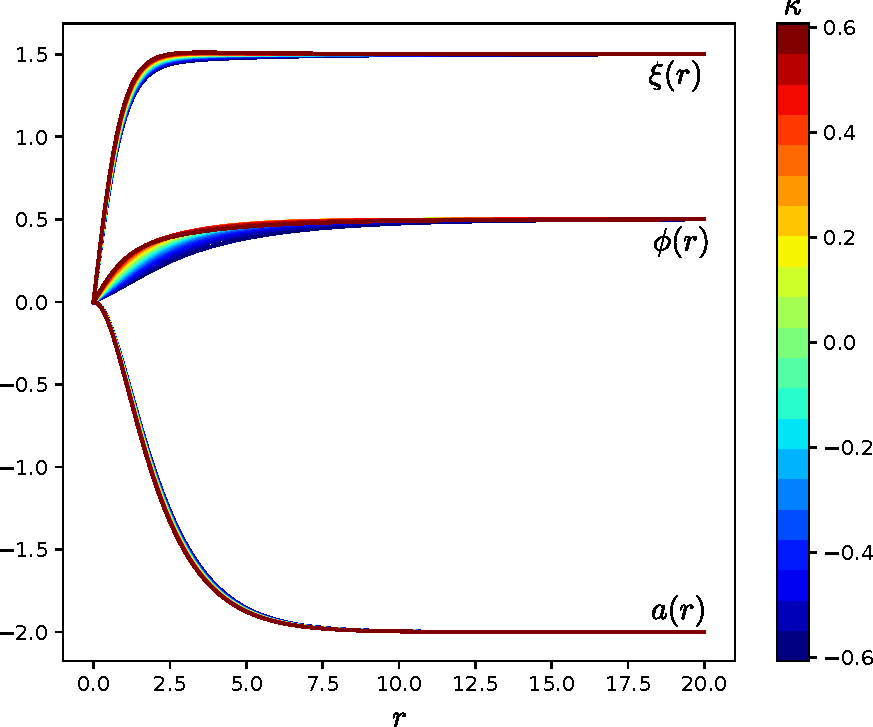
\includegraphics[scale=1]{./figures/Figure_2.pdf}
%\caption{$h=n=0$, $h'=n' = 1$, $\lambda=\lambda'=1$, $v=1/2$, $v'=1$ and $\kappa\in [-2,2]$.}
%\label{fig:2}
%\end{figure}
%
%\begin{figure}
%\centering
%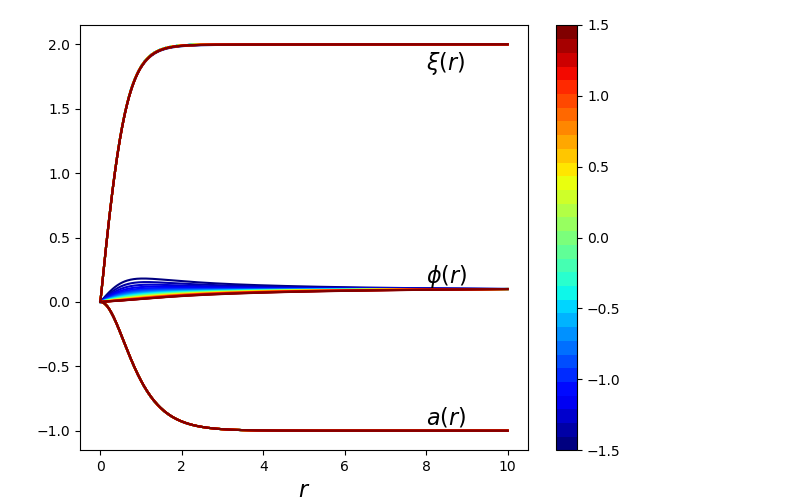
\includegraphics[scale=1]{./figures/Figure_3.png}
%\caption{$h=n=1$, $h'=n' = 1$, $\lambda=1, \lambda'=1/4$, $v=0.1$, $v'=2$ and $\kappa\in [-1.5,1.5]$.}
%\label{fig:3}
%\end{figure}
%
%\begin{figure}
%\centering
%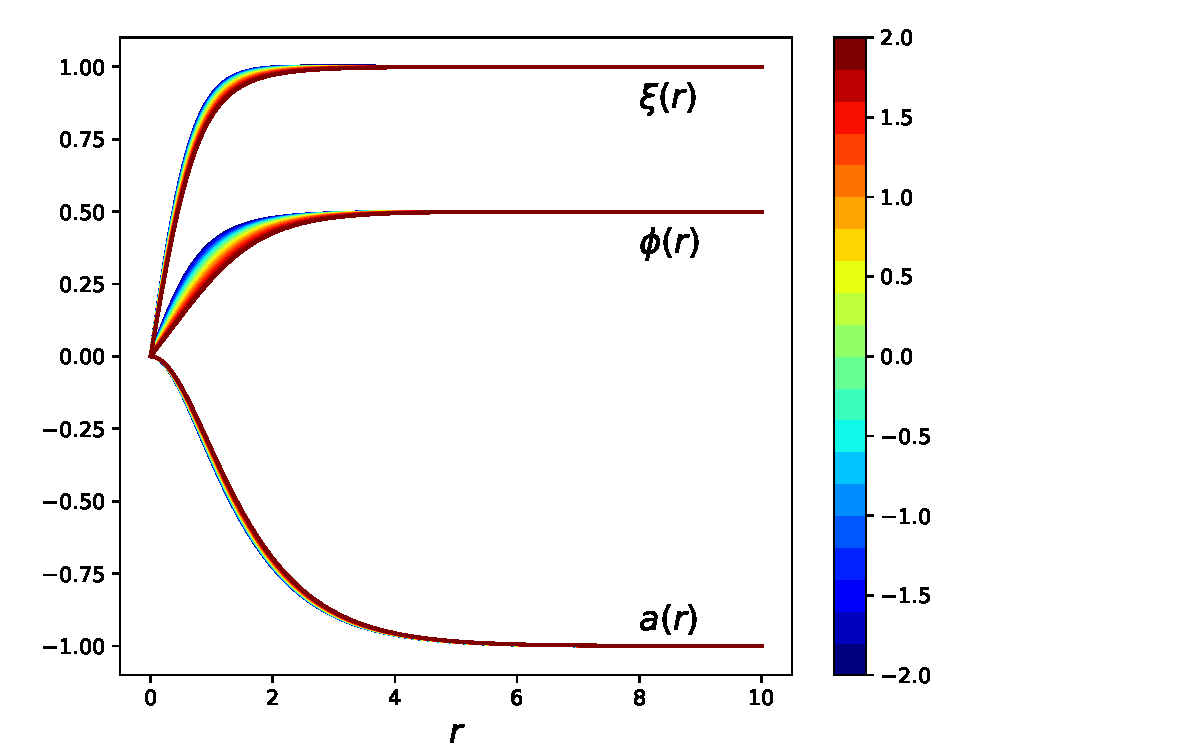
\includegraphics[scale=1]{./figures/Figure_4.pdf}
%\caption{$h=n=1$, $h'=n' = 1$, $\lambda=\lambda'=1$, $v=1/2$, $v'=1$ and $\kappa\in [-2,2]$.}
%\label{fig:4}
%\end{figure}
